\documentclass[aps,letterpaper,10pt]{revtex4}

\usepackage{multirow}
\usepackage{wrapfig}
\usepackage{graphicx} % For images
\usepackage{float}    % For tables and other floats
\usepackage{verbatim} % For comments and other
\usepackage{amsmath}  % For math
\usepackage{amssymb}  % For more math
\usepackage{fullpage} % Set margins and place page numbers at bottom center
\usepackage{listings} % For source code
\usepackage{subfig}   % For subfigures
\usepackage[usenames,dvipsnames]{color} % For colors and names
\usepackage[pdftex]{hyperref}           % For hyperlinks and indexing the PDF
\usepackage[svgnames]{xcolor}
\usepackage{tikz}
\usetikzlibrary{arrows,shapes,positioning}
\tikzstyle arrowstyle=[scale=1]
\tikzset{every node/.append style={minimum size=0.5cm, draw,circle}}
\hypersetup{ % play with the different link colors here
    colorlinks,
    citecolor=blue,
    filecolor=blue,
    linkcolor=blue,
    urlcolor=blue % set to black to prevent printing blue links
}

\definecolor{mygrey}{gray}{.96} % Light Grey
\lstset{
    language=[ISO]C++,              % choose the language of the code ("language=Verilog" is popular as well)
    tabsize=3,							  % sets the size of the tabs in spaces (1 Tab is replaced with 3 spaces)
    basicstyle=\tiny,               % the size of the fonts that are used for the code
    numbers=left,                   % where to put the line-numbers
    numberstyle=\tiny,              % the size of the fonts that are used for the line-numbers
    stepnumber=2,                   % the step between two line-numbers. If it's 1 each line will be numbered
    numbersep=5pt,                  % how far the line-numbers are from the code
    backgroundcolor=\color{mygrey}, % choose the background color. You must add \usepackage{color}
    %showspaces=false,              % show spaces adding particular underscores
    %showstringspaces=false,        % underline spaces within strings
    %showtabs=false,                % show tabs within strings adding particular underscores
    frame=single,	                 % adds a frame around the code
    tabsize=3,	                    % sets default tabsize to 2 spaces
    captionpos=b,                   % sets the caption-position to bottom
    breaklines=true,                % sets automatic line breaking
    breakatwhitespace=false,        % sets if automatic breaks should only happen at whitespace
    %escapeinside={\%*}{*)},        % if you want to add a comment within your code
    commentstyle=\color{BrickRed}   % sets the comment style
}

\newcommand{\labno}{05}
\newcommand{\labtitle}{AU 332 Artificial Intelligence: Principles and Techniques}
\newcommand{\authorname}{Guowei Deng}
\newcommand{\professor}{Yue Gao}

\begin{document}

\begin{titlepage}
\begin{center}
{\Large \textsc{\labtitle} \\ \vspace{4pt}}
\rule[13pt]{\textwidth}{1pt} \\ \vspace{150pt}
{\large By: \authorname \\ \vspace{10pt}
Instructor: \professor \\ \vspace{10pt}
\today}
\end{center}
\end{titlepage}
\section{Introduction}
\begin{center}
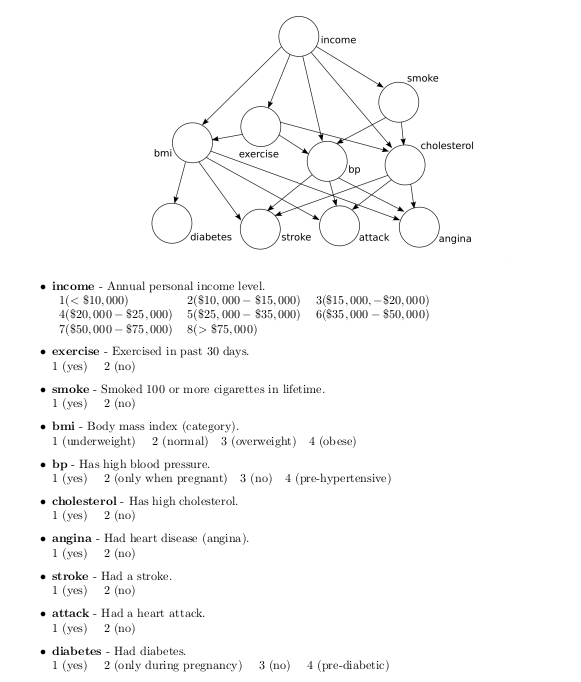
\includegraphics[scale=0.8]{graph.png}
\end{center}
The variables and their meanings are as above. In this lecture, we will be analyzing risk factors 
for certain health problems (heart disease, stroke, heart attack, diabetes) using data from the 2015 Behavioral Risk Factor Surveillance System (BRFSS) survey.
\newpage
\section{Problems}
\subsection{problem 1}
Simply, figure out parent nodes for every node. Then create a BayesNetwork using the given function \textbf{readFactorTablefromData}.
Compute the number of probabilities in every factor table.
Consequently, the number of probabilities needed of this network is 504. Alternatively, the total number of probabilities needed to store the full joint distribution should be $2^{15}$.
\subsection{problem 2}
The final result is as follows:
\begin{figure}[h]
\centering
\begin{minipage}[t]{0.5\linewidth}
    \centering
    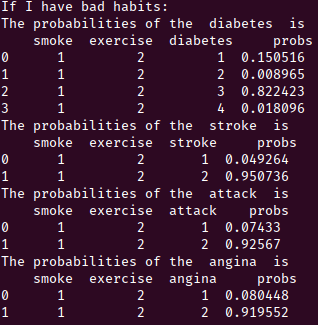
\includegraphics[scale=0.5]{2(a)(1).png}
    \caption{bad habits}
\end{minipage}%
\begin{minipage}[t]{0.5\linewidth}
    \centering
    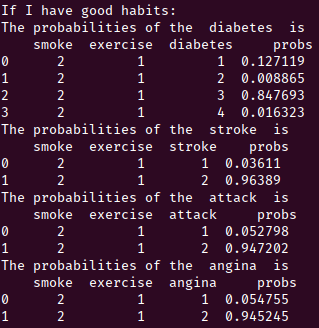
\includegraphics[scale=0.5]{2(a)(2).png}
    \caption{good habits}
\end{minipage}\\
\centering
\begin{minipage}[t]{0.5\linewidth}
    \centering
    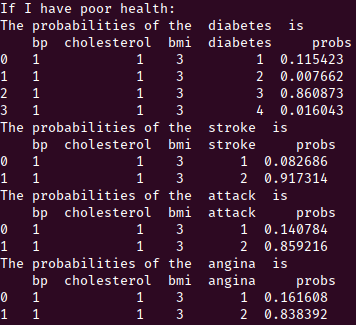
\includegraphics[scale=0.5]{2(b)(1).png}
    \caption{poor health}
\end{minipage}%
\begin{minipage}[t]{0.5\linewidth}
    \centering
    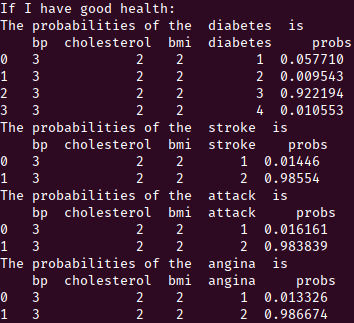
\includegraphics[scale=0.5]{2(b)(2).png}
    \caption{good health}
\end{minipage}
\end{figure}\\
\newpage
From the output of the code, we can learn:
\begin{table}[h]
\begin{tabular}{|c|c|c|c|c|c|}
    \hline
    \multicolumn{2}{|c|}{health outcomes}  & bad habits & good habits &poor health  &good health\\
    \hline
    \multirow{4}{*}{diabetes} &yes                 & 15.05\%     & 12.71\%    &11.54\%      &5.77\%  \\
    \cline{2-6}                    &only during pregncy & 0.89\%     & 0.88\%      &0.76\%       &0.95\%\\
    \cline{2-6}                       &no                  & 82.24\%     & 84.77\%    &86.08\%      &92.21\%\\
    \cline{2-6}                    &pre diabetic        & 1.81\%     & 1.63\%      &1.60\%       &1.05\%\\
    \hline
    \multirow{2}{*}{stroke}   &yes  & 4.92\%     & 3.61\%       &8.27\%       & 1.44\% \\
    \cline{2-6}                          &no   & 95.08\%    & 96.39\%      &91.73\%      & 98.56\%\\
    \hline
    \multirow{2}{*}{heart attack}   &yes        & 7.43\%     & 5.28\%       &14.08\%      & 1.61\%\\
    \cline{2-6}                     &no         & 92.57\%     & 94.72\%       &85.92\%      & 98.39\%\\
    \hline
    \multirow{2}{*}{angina}   &yes        & 8.04\%     & 5.47\%       &16.16\%      & 1.33\%\\
    \cline{2-6}               &no         & 91.96\%     & 94.53\%       &83.84\%      & 98.67\%\\
    \hline
\end{tabular}
\end{table}
\subsection{question3}
The probabilities of suffering from these 4 diseases for different 
income level is as follows:
\begin{center}
    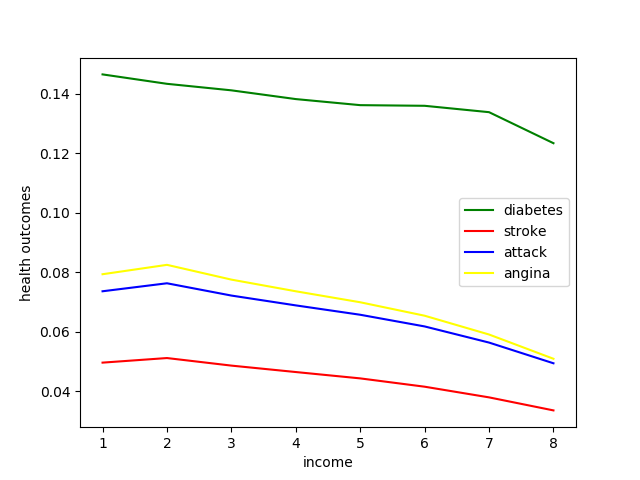
\includegraphics[scale=0.5]{3_figure.png}
\end{center}
\par
Generally, we can find that the higher a person's annual income level is, the less probabilities 
to suffer from these diseases. However, people who earn \$10000-\$15000(level 2) rather than level 1 seem to be more likely to 
suffer from these 4 diseases. In terms of different diseases, the probabilities in diabetes for different income is quite close. 
\newpage
\subsection{question4}
\begin{figure}[h]
    \centering
    \begin{minipage}[t]{0.45\linewidth}
        \centering
        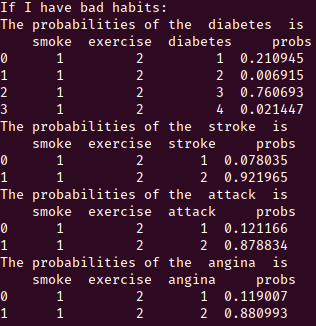
\includegraphics[scale=0.45]{4(a)(1).png}
        \caption{bad habits}
    \end{minipage}%
    \begin{minipage}[t]{0.45\linewidth}
        \centering
        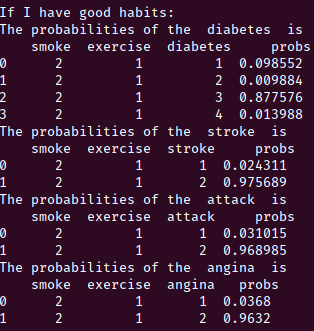
\includegraphics[scale=0.45]{4(a)(2).png}
        \caption{good habits}
    \end{minipage}\\
    \centering
    \begin{minipage}[t]{0.5\linewidth}
        \centering
        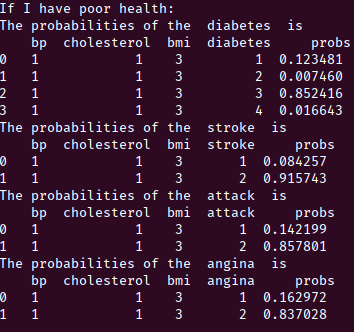
\includegraphics[scale=0.45]{4(b)(1).png}
        \caption{poor health}
    \end{minipage}%
    \begin{minipage}[t]{0.5\linewidth}
        \centering
        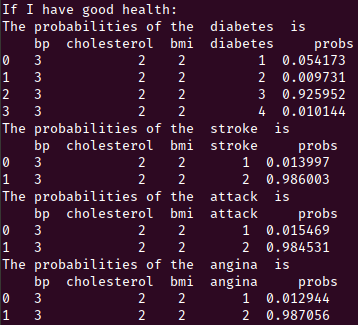
\includegraphics[scale=0.45]{4(b)(2).png}
        \caption{good health}
    \end{minipage}
\end{figure}
\begin{table}[h]
    \caption{first graph/second graph}
    \begin{tabular}{|c|c|c|c|c|c|}
        \hline
        \multicolumn{2}{|c|}{health outcomes}  & bad habits & good habits &poor health  &good health\\
        \hline
        \multirow{4}{*}{diabetes} &yes         & 15.05\%/21.09\%     & 12.71\%/9.85\%    &11.54\%/12.34\%      &5.77\%/5.41\%  \\
        \cline{2-6}                    &only during pregncy & 0.89\%/0.69\%     & 0.88\%/0.99\%      &0.76\%/0.75\%       &0.95\%/0.97\%\\
        \cline{2-6}                       &no                  & 82.24\%/76.06\%     & 84.77\%/87.75\%    &86.08\%85.24\%      &92.21\%/92.59\%\\
        \cline{2-6}                    &pre diabetic        & 1.81\%/2.14\%     & 1.63\%/1.40\%      &1.60\%/1.66\%       &1.05\%/1.01\%\\
        \hline
        \multirow{2}{*}{stroke}   &yes  & 4.92\%/7.80\%     & 3.61\%/2.43\%      &8.27\%8.42\%       & 1.44\%1.40\% \\
        \cline{2-6}                          &no   & 95.08\%/92.19\%    & 96.39\%/97.57\%      &91.73\%/91.57\%      & 98.56\%/98.60\%\\
        \hline
        \multirow{2}{*}{heart attack}   &yes        & 7.43\%/12.12\%     & 5.28\%/3.10\%       &14.08\%/14.21\%      & 1.61\%/1.55\%\\
        \cline{2-6}                     &no         & 92.57\%/87.88\%     & 94.72\%/96.89\%       &85.92\%/85.78\%      & 98.39\%/98.45\%\\
        \hline
        \multirow{2}{*}{angina}   &yes        & 8.04\%/11.90\%     & 5.47\%/3.68\%       &16.16\%/16.29\%      & 1.33\%/1.29\%\\
        \cline{2-6}               &no         & 91.96\%/88.10\%     & 94.53\%/96.32\%       &83.84\%/83.70\%      & 98.67\%/98.71\%\\
        \hline
    \end{tabular}
    \end{table}
After add edges, we can find that the probabilities in bad habits and good habits change a lot. However, the probabilities in poor health and good health in second graph is almost the same as 
the first graph. To clarify the relationship, we simplify the graph as follows:\\
\begin{center}
\begin{tikzpicture}[node distance=2cm]
    \node (income) [circle, ] {income};
    \node (health) [circle, below of= income] {health};
    \node (habits) [circle, left of = health] {habits};
    \node (outcomes) [circle, below of= health] {outcomes};
    \draw [->](income) -- (health);
    \draw [->](income) -- (habits);
    \draw [->](health) -- (outcomes);
    \draw [->](habits) -- (health);
    \draw [dashed, ->](habits) -- (outcomes);
\end{tikzpicture}
\end{center}
\par Giving health's value, habits and outcomes are conditional independent in first graph. After adding edges from habits to outcomes, 
the probabilities of outcomes won't change a lot, which means it's not worthwhile for us to add these edges. However, given habits' values, 
the probabilities of outcomes change a lot, which means there are some dependences between habits and outcomes. In conclude, I think the assumption 
in first graph is not valid. Without the edges from habits to outcomes, the graph is not accurate.
\subsection{question5}
\begin{center}
    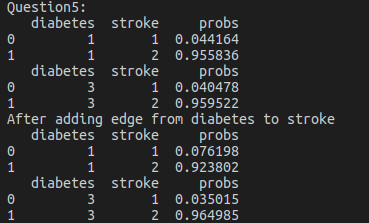
\includegraphics[scale=0.8]{5.png}
\end{center}
From the result below, we find that if a person has diabetes, it's much more likely that he or she has a stroke(7.61\% vs 4.41\%). So I think the interaction between diabetes and 
stroke are valid. 
\end{document}